\documentclass{extbook}[14pt]
\usepackage{multicol, enumerate, enumitem, hyperref, color, soul, setspace, parskip, fancyhdr, amssymb, amsthm, amsmath, latexsym, units, mathtools}
\everymath{\displaystyle}
\usepackage[headsep=0.5cm,headheight=0cm, left=1 in,right= 1 in,top= 1 in,bottom= 1 in]{geometry}
\usepackage{dashrule}  % Package to use the command below to create lines between items
\newcommand{\litem}[1]{\item #1

\rule{\textwidth}{0.4pt}}
\pagestyle{fancy}
\lhead{}
\chead{Answer Key for Module12L Version ALL}
\rhead{}
\lfoot{6131-5778}
\cfoot{}
\rfoot{test}
\begin{document}
\textbf{This key should allow you to understand why you choose the option you did (beyond just getting a question right or wrong). \href{https://xronos.clas.ufl.edu/mac1105spring2020/courseDescriptionAndMisc/Exams/LearningFromResults}{More instructions on how to use this key can be found here}.}

\textbf{If you have a suggestion to make the keys better, \href{https://forms.gle/CZkbZmPbC9XALEE88}{please fill out the short survey here}.}

\textit{Note: This key is auto-generated and may contain issues and/or errors. The keys are reviewed after each exam to ensure grading is done accurately. If there are issues (like duplicate options), they are noted in the offline gradebook. The keys are a work-in-progress to give students as many resources to improve as possible.}

\rule{\textwidth}{0.4pt}

\begin{enumerate}\litem{
Determine the horizontal and/or oblique asymptotes in the rational function below.
\[ f(x) = \frac{3x^{2} -13 x + 12}{12x^{3} -25 x^{2} -18 x + 40} \]The solution is \( \text{Horizontal Asymptote of } y = 0 \).\begin{enumerate}[label=\Alph*.]
\textbf{Plausible alternative answers include:}This corresponds to using rule for Horizontal Asymptote when degree of numerator and denominator match.
* This is the correct option.
This corresponds to considering where the denominator is equal to 0 as horizontal asymptote.
This corresponds to believing there can be both a horizontal and oblique asymptote.
This corresponds to flipping the numerator and denominator, then using synthetic division to find the oblique asymptote.
\end{enumerate}

\textbf{General Comment:} We have a Horizontal Asymptote if the degree of the numerator is smaller than or equal to the degree of the denominator. We have an Oblique Asymptote if the degree of the numerator is larger than the degree of the denominator. We cannot have both!
}
\litem{
Determine the horizontal and/or oblique asymptotes in the rational function below.
\[ f(x) = \frac{12x^{3} -13 x^{2} -19 x + 20}{-15x^{3} +52 x^{2} -48 x + 16} \]The solution is \( \text{Horizontal Asymptote of } y = -0.800  \).\begin{enumerate}[label=\Alph*.]
\textbf{Plausible alternative answers include:}This corresponds to believing there should be an oblique asymptote.
This corresponds to the hole at $x = 1$.
This corresponds to using the rule for Horizontal Asymptote when the degree of the denominator is larger than the numerator.
This corresponds to the hole at $x = 0.800$.
* This is the correct option.
\end{enumerate}

\textbf{General Comment:} We have a Horizontal Asymptote if the degree of the numerator is smaller than or equal to the degree of the denominator. We have an Oblique Asymptote if the degree of the numerator is larger than the degree of the denominator. We cannot have both!
}
\litem{
Determine the vertical asymptotes and holes in the rational function below.
\[ f(x) = \frac{12x^{3} +55 x^{2} +18 x -40}{12x^{2} -5 x -25} \]The solution is \( \text{Vertical Asymptote of } x = 1.667 \text{ and hole at } x = -1.25 \).\begin{enumerate}[label=\Alph*.]
\textbf{Plausible alternative answers include:}This corresponds to mixing vertical and horizontal asymptotes.
This corresponds to setting the numerator equal to 0.
This corresponds to not factoring out the hole.
This is the correct answer.
This corresponds to considering where the denominator is equal to 0 as holes.
\end{enumerate}

\textbf{General Comment:} Remember to factor the numerator and denominator. Any factors that cancel are holes in the function. The zeros left in the denominator are the vertical asymptotes.
}
\litem{
Write an equation of a function that \textit{could} be represented by the graph below. Explain why your function could represent the graph.

\begin{center}
    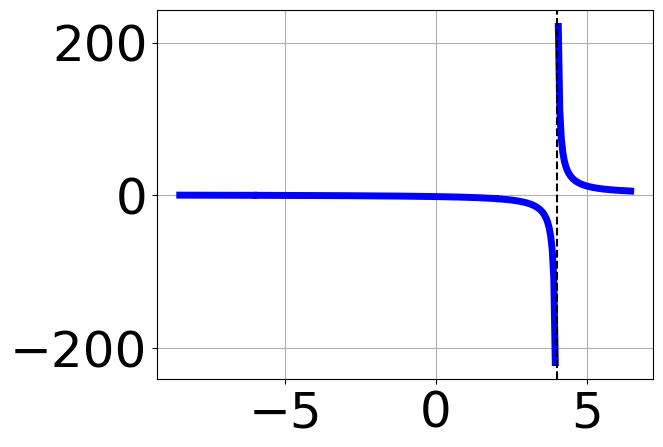
\includegraphics[width=0.5\textwidth]{../Figures/identifyGraphOfRationalFunctionA.png}
\end{center}


The solution is \( f(x)=\frac{x^{3} -2.0 x^{2} -23.0 x + 60.0}{x^{3} -9.0 x^{2} +26.0 x -24.0} \).\begin{enumerate}[label=\Alph*.]
\textbf{Plausible alternative answers include:}You treated all of the zeros in the denominator as vertical asymptotes when some of them were holes!
Remember that factors are written as $x-z$. For example, the zero $x=2$ corresponds to the factor $x-(2)$.
You treated all of the zeros in the denominator as vertical asmptotes when some of them were holes and wrote factors as $x+z$.
This is the correct answer!
If you believe none of the functions above could be the graph, please contact the coordinator.
\end{enumerate}

\textbf{General Comment:} We want to factor the numerator and denominator to determine which zeros in the denominator are vertical asympototes and which are holes.
}
\litem{
Write an equation of a function that \textit{could} be represented by the graph below. Explain why your function could represent the graph.

\begin{center}
    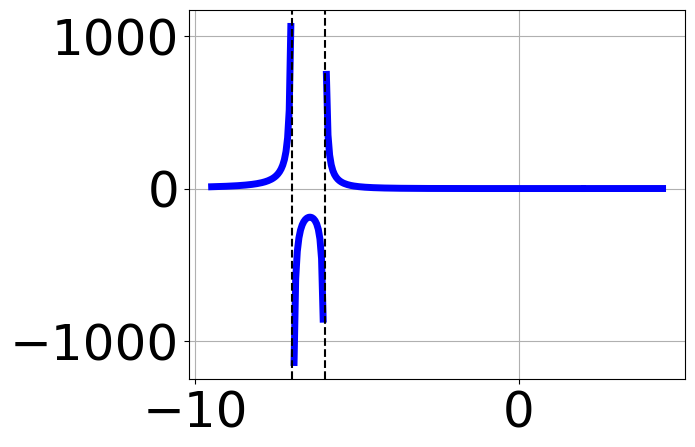
\includegraphics[width=0.5\textwidth]{../Figures/identifyGraphOfRationalFunctionCopyA.png}
\end{center}


The solution is \( f(x)=\frac{x^{3} -1.0 x^{2} -22.0 x + 40.0}{x^{3} -6.0 x^{2} +5.0 x + 12.0} \).\begin{enumerate}[label=\Alph*.]
\textbf{Plausible alternative answers include:}You treated all of the zeros in the denominator as vertical asmptotes when some of them were holes and wrote factors as $x+z$.
You treated all of the zeros in the denominator as vertical asymptotes when some of them were holes!
Remember that factors are written as $x-z$. For example, the zero $x=-1$ corresponds to the factor $x-(-1)$.
This is the correct answer!
If you believe none of the functions above could be the graph, please contact the coordinator.
\end{enumerate}

\textbf{General Comment:} We want to factor the numerator and denominator to determine which zeros in the denominator are vertical asympototes and which are holes.
}
\litem{
Determine the horizontal and/or oblique asymptotes in the rational function below.
\[ f(x) = \frac{6x^{3} +7 x^{2} -43 x -30}{2x^{2} +x -15} \]The solution is \( y = 3x + 2 \).\begin{enumerate}[label=\Alph*.]
\textbf{Plausible alternative answers include:}This is the correct answer.
This corresponds to believing there can be both a horizontal and oblique asymptote AND mixing up horizontal/vertical asymoptote.
This corresponds to using rule for Horizontal Asymptote when degree of numerator and denominator match.
This corresponds to believing there can be both a horizontal and oblique asymptote.
This corresponds to considering where the denominator is equal to 0 as horizontal asymptote.
\end{enumerate}

\textbf{General Comment:} We have a Horizontal Asymptote if the degree of the numerator is smaller than or equal to the degree of the denominator. We have an Oblique Asymptote if the degree of the numerator is larger than the degree of the denominator. We cannot have both!
}
\litem{
Determine the vertical asymptotes and holes in the rational function below.
\[ f(x) = \frac{4x^{3} +12 x^{2} -7 x -30}{6x^{2} -x -12} \]The solution is \( \text{Vertical Asymptote of } x = -1.333 \text{ and hole at } x = 1.5 \).\begin{enumerate}[label=\Alph*.]
\textbf{Plausible alternative answers include:}This corresponds to not factoring out the hole.
This corresponds to mixing vertical and horizontal asymptotes.
This corresponds to considering where the denominator is equal to 0 as holes.
This is the correct answer.
This corresponds to setting the numerator equal to 0.
\end{enumerate}

\textbf{General Comment:} Remember to factor the numerator and denominator. Any factors that cancel are holes in the function. The zeros left in the denominator are the vertical asymptotes.
}
\litem{
Determine the vertical asymptotes and holes in the rational function below.
\[ f(x) = \frac{6x^{3} -31 x^{2} +53 x -30}{12x^{2} -35 x + 25} \]The solution is \( \text{Vertical Asymptote of } x = 1.25 \text{ and hole at } x = 1.667 \).\begin{enumerate}[label=\Alph*.]
\textbf{Plausible alternative answers include:}This corresponds to mixing vertical and horizontal asymptotes.
This is the correct answer.
This corresponds to not factoring out the hole.
This corresponds to considering where the denominator is equal to 0 as holes.
This corresponds to setting the numerator equal to 0.
\end{enumerate}

\textbf{General Comment:} Remember to factor the numerator and denominator. Any factors that cancel are holes in the function. The zeros left in the denominator are the vertical asymptotes.
}
\litem{
Determine the vertical asymptotes and holes in the rational function below.
\[ f(x) = \frac{8x^{3} +6 x^{2} -17 x -15}{6x^{2} -17 x + 12} \]The solution is \( \text{Vertical Asymptote of } x = 1.333 \text{ and hole at } x = 1.5 \).\begin{enumerate}[label=\Alph*.]
\textbf{Plausible alternative answers include:}This corresponds to setting the numerator equal to 0.
This corresponds to considering where the denominator is equal to 0 as holes.
This corresponds to not factoring out the hole.
This corresponds to mixing vertical and horizontal asymptotes.
This is the correct answer.
\end{enumerate}

\textbf{General Comment:} Remember to factor the numerator and denominator. Any factors that cancel are holes in the function. The zeros left in the denominator are the vertical asymptotes.
}
\litem{
Determine the horizontal and/or oblique asymptotes in the rational function below.
\[ f(x) = \frac{6x^{3} + x^{2} -27 x + 20}{2x^{2} +11 x + 15} \]The solution is \( y = 3x -16 \).\begin{enumerate}[label=\Alph*.]
\textbf{Plausible alternative answers include:}This corresponds to believing there can be both a horizontal and oblique asymptote.
This corresponds to believing there can be both a horizontal and oblique asymptote AND mixing up horizontal/vertical asymoptote.
This corresponds to using rule for Horizontal Asymptote when degree of numerator and denominator match.
This corresponds to considering where the denominator is equal to 0 as horizontal asymptote.
This is the correct answer.
\end{enumerate}

\textbf{General Comment:} We have a Horizontal Asymptote if the degree of the numerator is smaller than or equal to the degree of the denominator. We have an Oblique Asymptote if the degree of the numerator is larger than the degree of the denominator. We cannot have both!
}
\litem{
Determine the horizontal and/or oblique asymptotes in the rational function below.
\[ f(x) = \frac{9x^{3} -9 x^{2} -88 x -80}{6x^{3} + x^{2} +8 x + 80} \]The solution is \( \text{Horizontal Asymptote of } y = 1.500  \).\begin{enumerate}[label=\Alph*.]
\textbf{Plausible alternative answers include:}* This is the correct option.
This corresponds to believing there should be an oblique asymptote.
This corresponds to the hole at $x = 4$.
This corresponds to the hole at $x = 2.500$.
This corresponds to using the rule for Horizontal Asymptote when the degree of the denominator is larger than the numerator.
\end{enumerate}

\textbf{General Comment:} We have a Horizontal Asymptote if the degree of the numerator is smaller than or equal to the degree of the denominator. We have an Oblique Asymptote if the degree of the numerator is larger than the degree of the denominator. We cannot have both!
}
\litem{
Determine the horizontal and/or oblique asymptotes in the rational function below.
\[ f(x) = \frac{20x^{3} -33 x^{2} -2 x + 15}{20x^{3} -62 x^{2} +52 x -15} \]The solution is \( \text{Horizontal Asymptote of } y = 1.000  \).\begin{enumerate}[label=\Alph*.]
\textbf{Plausible alternative answers include:}This corresponds to using the rule for Horizontal Asymptote when the degree of the denominator is larger than the numerator.
This corresponds to believing there should be an oblique asymptote.
This corresponds to the hole at $x = 0.600$.
This corresponds to the hole at $x = 1$.
* This is the correct option.
\end{enumerate}

\textbf{General Comment:} We have a Horizontal Asymptote if the degree of the numerator is smaller than or equal to the degree of the denominator. We have an Oblique Asymptote if the degree of the numerator is larger than the degree of the denominator. We cannot have both!
}
\litem{
Determine the vertical asymptotes and holes in the rational function below.
\[ f(x) = \frac{8x^{3} -10 x^{2} -9 x + 9}{6x^{2} -5 x -6} \]The solution is \( \text{Vertical Asymptote of } x = -0.667 \text{ and hole at } x = 1.5 \).\begin{enumerate}[label=\Alph*.]
\textbf{Plausible alternative answers include:}This corresponds to not factoring out the hole.
This is the correct answer.
This corresponds to setting the numerator equal to 0.
This corresponds to considering where the denominator is equal to 0 as holes.
This corresponds to mixing vertical and horizontal asymptotes.
\end{enumerate}

\textbf{General Comment:} Remember to factor the numerator and denominator. Any factors that cancel are holes in the function. The zeros left in the denominator are the vertical asymptotes.
}
\litem{
Write an equation of a function that \textit{could} be represented by the graph below. Explain why your function could represent the graph.

\begin{center}
    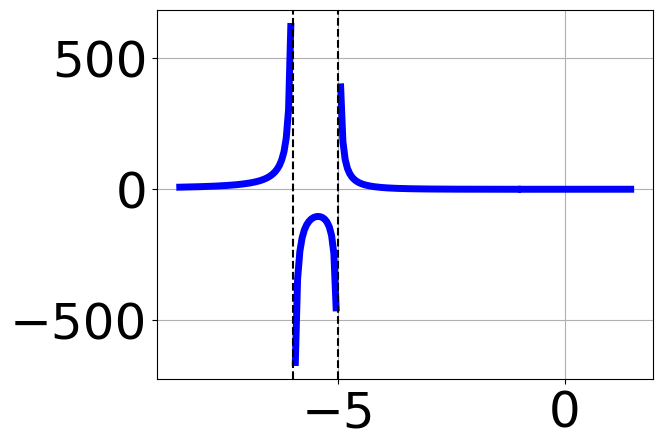
\includegraphics[width=0.5\textwidth]{../Figures/identifyGraphOfRationalFunctionB.png}
\end{center}


The solution is \( f(x)=\frac{x^{3} -5.0 x^{2} -x + 5.0}{x^{3} -9.0 x^{2} +23.0 x -15.0} \).\begin{enumerate}[label=\Alph*.]
\textbf{Plausible alternative answers include:}This is the correct answer!
You treated all of the zeros in the denominator as vertical asmptotes when some of them were holes and wrote factors as $x+z$.
You treated all of the zeros in the denominator as vertical asymptotes when some of them were holes!
Remember that factors are written as $x-z$. For example, the zero $x=3$ corresponds to the factor $x-(3)$.
If you believe none of the functions above could be the graph, please contact the coordinator.
\end{enumerate}

\textbf{General Comment:} We want to factor the numerator and denominator to determine which zeros in the denominator are vertical asympototes and which are holes.
}
\litem{
Write an equation of a function that \textit{could} be represented by the graph below. Explain why your function could represent the graph.

\begin{center}
    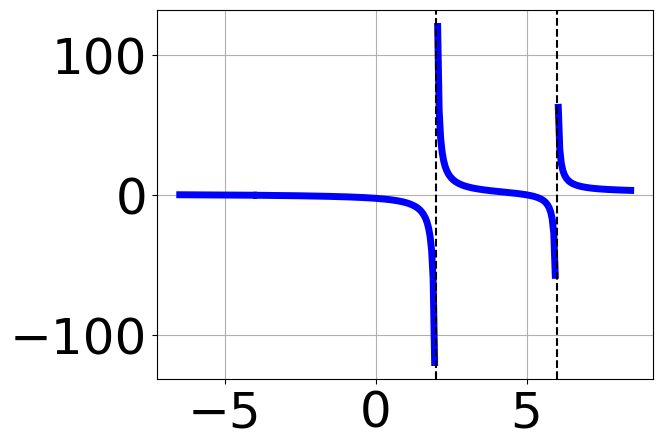
\includegraphics[width=0.5\textwidth]{../Figures/identifyGraphOfRationalFunctionCopyB.png}
\end{center}


The solution is \( f(x)=\frac{x^{3} +4.0 x^{2} -25.0 x -28.0}{x^{3} +7.0 x^{2} -14.0 x -120.0} \).\begin{enumerate}[label=\Alph*.]
\textbf{Plausible alternative answers include:}You treated all of the zeros in the denominator as vertical asymptotes when some of them were holes!
This is the correct answer!
You treated all of the zeros in the denominator as vertical asmptotes when some of them were holes and wrote factors as $x+z$.
Remember that factors are written as $x-z$. For example, the zero $x=-6$ corresponds to the factor $x-(-6)$.
If you believe none of the functions above could be the graph, please contact the coordinator.
\end{enumerate}

\textbf{General Comment:} We want to factor the numerator and denominator to determine which zeros in the denominator are vertical asympototes and which are holes.
}
\litem{
Determine the horizontal and/or oblique asymptotes in the rational function below.
\[ f(x) = \frac{8x^{3} -10 x^{2} -73 x -60}{4x^{2} +21 x + 20} \]The solution is \( y = 2x -13 \).\begin{enumerate}[label=\Alph*.]
\textbf{Plausible alternative answers include:}This corresponds to believing there can be both a horizontal and oblique asymptote AND mixing up horizontal/vertical asymoptote.
This corresponds to believing there can be both a horizontal and oblique asymptote.
This is the correct answer.
This corresponds to using rule for Horizontal Asymptote when degree of numerator and denominator match.
This corresponds to considering where the denominator is equal to 0 as horizontal asymptote.
\end{enumerate}

\textbf{General Comment:} We have a Horizontal Asymptote if the degree of the numerator is smaller than or equal to the degree of the denominator. We have an Oblique Asymptote if the degree of the numerator is larger than the degree of the denominator. We cannot have both!
}
\litem{
Determine the vertical asymptotes and holes in the rational function below.
\[ f(x) = \frac{12x^{3} -47 x^{2} +60 x -25}{9x^{2} -27 x + 20} \]The solution is \( \text{Vertical Asymptote of } x = 1.333 \text{ and hole at } x = 1.667 \).\begin{enumerate}[label=\Alph*.]
\textbf{Plausible alternative answers include:}This corresponds to considering where the denominator is equal to 0 as holes.
This corresponds to not factoring out the hole.
This corresponds to mixing vertical and horizontal asymptotes.
This corresponds to setting the numerator equal to 0.
This is the correct answer.
\end{enumerate}

\textbf{General Comment:} Remember to factor the numerator and denominator. Any factors that cancel are holes in the function. The zeros left in the denominator are the vertical asymptotes.
}
\litem{
Determine the vertical asymptotes and holes in the rational function below.
\[ f(x) = \frac{9x^{3} +36 x^{2} -25 x -100}{12x^{2} +29 x + 15} \]The solution is \( \text{Vertical Asymptote of } x = -0.75 \text{ and hole at } x = -1.667 \).\begin{enumerate}[label=\Alph*.]
\textbf{Plausible alternative answers include:}This corresponds to considering where the denominator is equal to 0 as holes.
This corresponds to not factoring out the hole.
This is the correct answer.
This corresponds to setting the numerator equal to 0.
This corresponds to mixing vertical and horizontal asymptotes.
\end{enumerate}

\textbf{General Comment:} Remember to factor the numerator and denominator. Any factors that cancel are holes in the function. The zeros left in the denominator are the vertical asymptotes.
}
\litem{
Determine the vertical asymptotes and holes in the rational function below.
\[ f(x) = \frac{8x^{3} -46 x^{2} +81 x -45}{16x^{2} -25} \]The solution is \( \text{Vertical Asymptote of } x = -1.25 \text{ and hole at } x = 1.25 \).\begin{enumerate}[label=\Alph*.]
\textbf{Plausible alternative answers include:}This corresponds to mixing vertical and horizontal asymptotes.
This corresponds to setting the numerator equal to 0.
This corresponds to considering where the denominator is equal to 0 as holes.
This corresponds to not factoring out the hole.
This is the correct answer.
\end{enumerate}

\textbf{General Comment:} Remember to factor the numerator and denominator. Any factors that cancel are holes in the function. The zeros left in the denominator are the vertical asymptotes.
}
\litem{
Determine the horizontal and/or oblique asymptotes in the rational function below.
\[ f(x) = \frac{6x^{3} -35 x^{2} +34 x + 40}{3x^{2} +17 x + 10} \]The solution is \( y = 2x -23 \).\begin{enumerate}[label=\Alph*.]
\textbf{Plausible alternative answers include:}This corresponds to believing there can be both a horizontal and oblique asymptote.
This corresponds to considering where the denominator is equal to 0 as horizontal asymptote.
This is the correct answer.
This corresponds to believing there can be both a horizontal and oblique asymptote AND mixing up horizontal/vertical asymoptote.
This corresponds to using rule for Horizontal Asymptote when degree of numerator and denominator match.
\end{enumerate}

\textbf{General Comment:} We have a Horizontal Asymptote if the degree of the numerator is smaller than or equal to the degree of the denominator. We have an Oblique Asymptote if the degree of the numerator is larger than the degree of the denominator. We cannot have both!
}
\litem{
Determine the horizontal and/or oblique asymptotes in the rational function below.
\[ f(x) = \frac{12x^{3} -53 x^{2} +57 x -18}{-12x^{3} +7 x^{2} +9 x -18} \]The solution is \( \text{Horizontal Asymptote of } y = -1.000  \).\begin{enumerate}[label=\Alph*.]
\textbf{Plausible alternative answers include:}This corresponds to believing there should be an oblique asymptote.
This corresponds to using the rule for Horizontal Asymptote when the degree of the denominator is larger than the numerator.
* This is the correct option.
This corresponds to the hole at $x = -0.750$.
This corresponds to the hole at $x = 3$.
\end{enumerate}

\textbf{General Comment:} We have a Horizontal Asymptote if the degree of the numerator is smaller than or equal to the degree of the denominator. We have an Oblique Asymptote if the degree of the numerator is larger than the degree of the denominator. We cannot have both!
}
\litem{
Determine the horizontal and/or oblique asymptotes in the rational function below.
\[ f(x) = \frac{9x^{3} +24 x^{2} -29 x -60}{-6x^{3} +32 x^{2} +46 x -60} \]The solution is \( \text{Horizontal Asymptote of } y = -1.500  \).\begin{enumerate}[label=\Alph*.]
\textbf{Plausible alternative answers include:}This corresponds to the hole at $x = 2.000$.
This corresponds to the hole at $x = -3$.
This corresponds to using the rule for Horizontal Asymptote when the degree of the denominator is larger than the numerator.
This corresponds to believing there should be an oblique asymptote.
* This is the correct option.
\end{enumerate}

\textbf{General Comment:} We have a Horizontal Asymptote if the degree of the numerator is smaller than or equal to the degree of the denominator. We have an Oblique Asymptote if the degree of the numerator is larger than the degree of the denominator. We cannot have both!
}
\litem{
Determine the vertical asymptotes and holes in the rational function below.
\[ f(x) = \frac{6x^{3} -1 x^{2} -47 x + 30}{6x^{2} -11 x -10} \]The solution is \( \text{Vertical Asymptote of } x = -0.667 \text{ and hole at } x = 2.5 \).\begin{enumerate}[label=\Alph*.]
\textbf{Plausible alternative answers include:}This corresponds to setting the numerator equal to 0.
This corresponds to mixing vertical and horizontal asymptotes.
This corresponds to not factoring out the hole.
This corresponds to considering where the denominator is equal to 0 as holes.
This is the correct answer.
\end{enumerate}

\textbf{General Comment:} Remember to factor the numerator and denominator. Any factors that cancel are holes in the function. The zeros left in the denominator are the vertical asymptotes.
}
\litem{
Write an equation of a function that \textit{could} be represented by the graph below. Explain why your function could represent the graph.

\begin{center}
    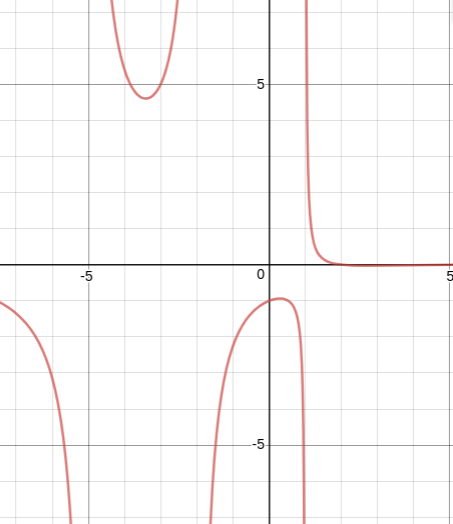
\includegraphics[width=0.5\textwidth]{../Figures/identifyGraphOfRationalFunctionC.png}
\end{center}


The solution is \( f(x)=\frac{x^{3} -3.0 x^{2} -36.0 x + 108.0}{x^{3} +3.0 x^{2} -36.0 x -108.0} \).\begin{enumerate}[label=\Alph*.]
\textbf{Plausible alternative answers include:}You treated all of the zeros in the denominator as vertical asmptotes when some of them were holes and wrote factors as $x+z$.
You treated all of the zeros in the denominator as vertical asymptotes when some of them were holes!
Remember that factors are written as $x-z$. For example, the zero $x=-3$ corresponds to the factor $x-(-3)$.
This is the correct answer!
If you believe none of the functions above could be the graph, please contact the coordinator.
\end{enumerate}

\textbf{General Comment:} We want to factor the numerator and denominator to determine which zeros in the denominator are vertical asympototes and which are holes.
}
\litem{
Write an equation of a function that \textit{could} be represented by the graph below. Explain why your function could represent the graph.

\begin{center}
    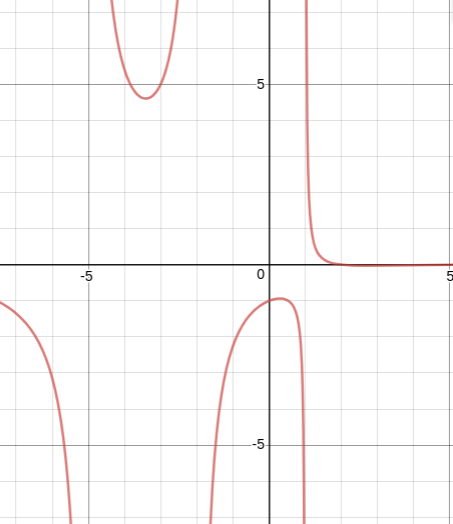
\includegraphics[width=0.5\textwidth]{../Figures/identifyGraphOfRationalFunctionCopyC.png}
\end{center}


The solution is \( f(x)=\frac{x^{3} +7.0 x^{2} -x -7.0}{x^{3} -3.0 x^{2} -x + 3.0} \).\begin{enumerate}[label=\Alph*.]
\textbf{Plausible alternative answers include:}You treated all of the zeros in the denominator as vertical asmptotes when some of them were holes and wrote factors as $x+z$.
You treated all of the zeros in the denominator as vertical asymptotes when some of them were holes!
Remember that factors are written as $x-z$. For example, the zero $x=3$ corresponds to the factor $x-(3)$.
This is the correct answer!
If you believe none of the functions above could be the graph, please contact the coordinator.
\end{enumerate}

\textbf{General Comment:} We want to factor the numerator and denominator to determine which zeros in the denominator are vertical asympototes and which are holes.
}
\litem{
Determine the horizontal and/or oblique asymptotes in the rational function below.
\[ f(x) = \frac{6x^{3} -29 x^{2} +23 x + 30}{3x^{2} -13 x -10} \]The solution is \( y = 2x -1 \).\begin{enumerate}[label=\Alph*.]
\textbf{Plausible alternative answers include:}This is the correct answer.
This corresponds to considering where the denominator is equal to 0 as horizontal asymptote.
This corresponds to believing there can be both a horizontal and oblique asymptote AND mixing up horizontal/vertical asymoptote.
This corresponds to believing there can be both a horizontal and oblique asymptote.
This corresponds to using rule for Horizontal Asymptote when degree of numerator and denominator match.
\end{enumerate}

\textbf{General Comment:} We have a Horizontal Asymptote if the degree of the numerator is smaller than or equal to the degree of the denominator. We have an Oblique Asymptote if the degree of the numerator is larger than the degree of the denominator. We cannot have both!
}
\litem{
Determine the vertical asymptotes and holes in the rational function below.
\[ f(x) = \frac{12x^{3} -59 x^{2} +95 x -50}{9x^{2} -25} \]The solution is \( \text{Vertical Asymptote of } x = -1.667 \text{ and hole at } x = 1.667 \).\begin{enumerate}[label=\Alph*.]
\textbf{Plausible alternative answers include:}This corresponds to setting the numerator equal to 0.
This corresponds to not factoring out the hole.
This corresponds to considering where the denominator is equal to 0 as holes.
This corresponds to mixing vertical and horizontal asymptotes.
This is the correct answer.
\end{enumerate}

\textbf{General Comment:} Remember to factor the numerator and denominator. Any factors that cancel are holes in the function. The zeros left in the denominator are the vertical asymptotes.
}
\litem{
Determine the vertical asymptotes and holes in the rational function below.
\[ f(x) = \frac{9x^{3} +15 x^{2} -2 x -8}{9x^{2} -18 x + 8} \]The solution is \( \text{Vertical Asymptote of } x = 1.333 \text{ and hole at } x = 0.667 \).\begin{enumerate}[label=\Alph*.]
\textbf{Plausible alternative answers include:}This corresponds to not factoring out the hole.
This corresponds to setting the numerator equal to 0.
This corresponds to mixing vertical and horizontal asymptotes.
This is the correct answer.
This corresponds to considering where the denominator is equal to 0 as holes.
\end{enumerate}

\textbf{General Comment:} Remember to factor the numerator and denominator. Any factors that cancel are holes in the function. The zeros left in the denominator are the vertical asymptotes.
}
\litem{
Determine the vertical asymptotes and holes in the rational function below.
\[ f(x) = \frac{6x^{3} +49 x^{2} +125 x + 100}{9x^{2} +27 x + 20} \]The solution is \( \text{Vertical Asymptote of } x = -1.333 \text{ and hole at } x = -1.667 \).\begin{enumerate}[label=\Alph*.]
\textbf{Plausible alternative answers include:}This corresponds to not factoring out the hole.
This is the correct answer.
This corresponds to mixing vertical and horizontal asymptotes.
This corresponds to considering where the denominator is equal to 0 as holes.
This corresponds to setting the numerator equal to 0.
\end{enumerate}

\textbf{General Comment:} Remember to factor the numerator and denominator. Any factors that cancel are holes in the function. The zeros left in the denominator are the vertical asymptotes.
}
\litem{
Determine the horizontal and/or oblique asymptotes in the rational function below.
\[ f(x) = \frac{6x^{3} +13 x^{2} -9 x -10}{3x^{2} -10 x -8} \]The solution is \( y = 2x + 11 \).\begin{enumerate}[label=\Alph*.]
\textbf{Plausible alternative answers include:}This corresponds to believing there can be both a horizontal and oblique asymptote.
This corresponds to considering where the denominator is equal to 0 as horizontal asymptote.
This corresponds to using rule for Horizontal Asymptote when degree of numerator and denominator match.
This is the correct answer.
This corresponds to believing there can be both a horizontal and oblique asymptote AND mixing up horizontal/vertical asymoptote.
\end{enumerate}

\textbf{General Comment:} We have a Horizontal Asymptote if the degree of the numerator is smaller than or equal to the degree of the denominator. We have an Oblique Asymptote if the degree of the numerator is larger than the degree of the denominator. We cannot have both!
}
\end{enumerate}

\end{document}